%%
%% Automatically generated file from DocOnce source
%% (https://github.com/hplgit/doconce/)
%%

% #define PREAMBLE

% #ifdef PREAMBLE
%-------------------- begin preamble ----------------------

\documentclass[%
oneside,                 % oneside: electronic viewing, twoside: printing
final,                   % draft: marks overfull hboxes, figures with paths
10pt]{article}

\listfiles               %  print all files needed to compile this document

\usepackage{relsize,makeidx,color,setspace,amsmath,amsfonts,amssymb}
\usepackage[table]{xcolor}
\usepackage{bm,ltablex,microtype}

\usepackage[pdftex]{graphicx}

\usepackage[T1]{fontenc}
%\usepackage[latin1]{inputenc}
\usepackage{ucs}
\usepackage[utf8x]{inputenc}

\usepackage{lmodern}         % Latin Modern fonts derived from Computer Modern

% Hyperlinks in PDF:
\definecolor{linkcolor}{rgb}{0,0,0.4}
\usepackage{hyperref}
\hypersetup{
    breaklinks=true,
    colorlinks=true,
    linkcolor=linkcolor,
    urlcolor=linkcolor,
    citecolor=black,
    filecolor=black,
    %filecolor=blue,
    pdfmenubar=true,
    pdftoolbar=true,
    bookmarksdepth=3   % Uncomment (and tweak) for PDF bookmarks with more levels than the TOC
    }
%\hyperbaseurl{}   % hyperlinks are relative to this root

\setcounter{tocdepth}{2}  % levels in table of contents

% Tricks for having figures close to where they are defined:
% 1. define less restrictive rules for where to put figures
\setcounter{topnumber}{2}
\setcounter{bottomnumber}{2}
\setcounter{totalnumber}{4}
\renewcommand{\topfraction}{0.95}
\renewcommand{\bottomfraction}{0.95}
\renewcommand{\textfraction}{0}
\renewcommand{\floatpagefraction}{0.75}
% floatpagefraction must always be less than topfraction!
% 2. ensure all figures are flushed before next section
\usepackage[section]{placeins}
% 3. enable begin{figure}[H] (often leads to ugly pagebreaks)
%\usepackage{float}\restylefloat{figure}

% --- fancyhdr package for fancy headers ---
\usepackage{fancyhdr}
\fancyhf{} % sets both header and footer to nothing
\renewcommand{\headrulewidth}{0pt}
\fancyfoot[LE,RO]{\thepage}
% Ensure copyright on titlepage (article style) and chapter pages (book style)
\fancypagestyle{plain}{
  \fancyhf{}
  \fancyfoot[C]{{\footnotesize \copyright\ 2018-2019, Christian Forssén. Released under CC Attribution-NonCommercial 4.0 license}}
%  \renewcommand{\footrulewidth}{0mm}
  \renewcommand{\headrulewidth}{0mm}
}
% Ensure copyright on titlepages with \thispagestyle{empty}
\fancypagestyle{empty}{
  \fancyhf{}
  \fancyfoot[C]{{\footnotesize \copyright\ 2018-2019, Christian Forssén. Released under CC Attribution-NonCommercial 4.0 license}}
  \renewcommand{\footrulewidth}{0mm}
  \renewcommand{\headrulewidth}{0mm}
}

\pagestyle{fancy}


\usepackage[framemethod=TikZ]{mdframed}

% --- begin definitions of admonition environments ---

% Admonition style "mdfbox" is an oval colored box based on mdframed
% "notice" admon
\definecolor{mdfbox_notice_background}{rgb}{1,1,1}
\newmdenv[
  skipabove=15pt,
  skipbelow=15pt,
  outerlinewidth=0,
  backgroundcolor=mdfbox_notice_background,
  linecolor=black,
  linewidth=2pt,       % frame thickness
  frametitlebackgroundcolor=mdfbox_notice_background,
  frametitlerule=true,
  frametitlefont=\normalfont\bfseries,
  shadow=false,        % frame shadow?
  shadowsize=11pt,
  leftmargin=0,
  rightmargin=0,
  roundcorner=5,
  needspace=0pt,
]{notice_mdfboxmdframed}

\newenvironment{notice_mdfboxadmon}[1][]{
\begin{notice_mdfboxmdframed}[frametitle=#1]
}
{
\end{notice_mdfboxmdframed}
}

% Admonition style "mdfbox" is an oval colored box based on mdframed
% "summary" admon
\definecolor{mdfbox_summary_background}{rgb}{1,1,1}
\newmdenv[
  skipabove=15pt,
  skipbelow=15pt,
  outerlinewidth=0,
  backgroundcolor=mdfbox_summary_background,
  linecolor=black,
  linewidth=2pt,       % frame thickness
  frametitlebackgroundcolor=mdfbox_summary_background,
  frametitlerule=true,
  frametitlefont=\normalfont\bfseries,
  shadow=false,        % frame shadow?
  shadowsize=11pt,
  leftmargin=0,
  rightmargin=0,
  roundcorner=5,
  needspace=0pt,
]{summary_mdfboxmdframed}

\newenvironment{summary_mdfboxadmon}[1][]{
\begin{summary_mdfboxmdframed}[frametitle=#1]
}
{
\end{summary_mdfboxmdframed}
}

% Admonition style "mdfbox" is an oval colored box based on mdframed
% "warning" admon
\definecolor{mdfbox_warning_background}{rgb}{1,1,1}
\newmdenv[
  skipabove=15pt,
  skipbelow=15pt,
  outerlinewidth=0,
  backgroundcolor=mdfbox_warning_background,
  linecolor=black,
  linewidth=2pt,       % frame thickness
  frametitlebackgroundcolor=mdfbox_warning_background,
  frametitlerule=true,
  frametitlefont=\normalfont\bfseries,
  shadow=false,        % frame shadow?
  shadowsize=11pt,
  leftmargin=0,
  rightmargin=0,
  roundcorner=5,
  needspace=0pt,
]{warning_mdfboxmdframed}

\newenvironment{warning_mdfboxadmon}[1][]{
\begin{warning_mdfboxmdframed}[frametitle=#1]
}
{
\end{warning_mdfboxmdframed}
}

% Admonition style "mdfbox" is an oval colored box based on mdframed
% "question" admon
\definecolor{mdfbox_question_background}{rgb}{1,1,1}
\newmdenv[
  skipabove=15pt,
  skipbelow=15pt,
  outerlinewidth=0,
  backgroundcolor=mdfbox_question_background,
  linecolor=black,
  linewidth=2pt,       % frame thickness
  frametitlebackgroundcolor=mdfbox_question_background,
  frametitlerule=true,
  frametitlefont=\normalfont\bfseries,
  shadow=false,        % frame shadow?
  shadowsize=11pt,
  leftmargin=0,
  rightmargin=0,
  roundcorner=5,
  needspace=0pt,
]{question_mdfboxmdframed}

\newenvironment{question_mdfboxadmon}[1][]{
\begin{question_mdfboxmdframed}[frametitle=#1]
}
{
\end{question_mdfboxmdframed}
}

% Admonition style "mdfbox" is an oval colored box based on mdframed
% "block" admon
\definecolor{mdfbox_block_background}{rgb}{1,1,1}
\newmdenv[
  skipabove=15pt,
  skipbelow=15pt,
  outerlinewidth=0,
  backgroundcolor=mdfbox_block_background,
  linecolor=black,
  linewidth=2pt,       % frame thickness
  frametitlebackgroundcolor=mdfbox_block_background,
  frametitlerule=true,
  frametitlefont=\normalfont\bfseries,
  shadow=false,        % frame shadow?
  shadowsize=11pt,
  leftmargin=0,
  rightmargin=0,
  roundcorner=5,
  needspace=0pt,
]{block_mdfboxmdframed}

\newenvironment{block_mdfboxadmon}[1][]{
\begin{block_mdfboxmdframed}[frametitle=#1]
}
{
\end{block_mdfboxmdframed}
}

% --- end of definitions of admonition environments ---

% prevent orhpans and widows
\clubpenalty = 10000
\widowpenalty = 10000

% --- end of standard preamble for documents ---


\usepackage[swedish]{babel}

\raggedbottom
\makeindex
\usepackage[totoc]{idxlayout}   % for index in the toc
\usepackage[nottoc]{tocbibind}  % for references/bibliography in the toc

%-------------------- end preamble ----------------------

\begin{document}

% matching end for #ifdef PREAMBLE
% #endif

\newcommand{\exercisesection}[1]{\subsection*{#1}}

\input{newcommands_keep}

% ------------------- main content ----------------------



% ----------------- title -------------------------

\thispagestyle{empty}

\begin{center}
{\LARGE\bf
\begin{spacing}{1.25}
Learning from data: Getting started and a first data and machine learning encounter
\end{spacing}
}
\end{center}

% ----------------- author(s) -------------------------

\begin{center}
{\bf Christian Forssén${}^{1}$} \\ [0mm]
\end{center}


\begin{center}
{\bf Morten Hjorth-Jensen${}^{2, 3}$} \\ [0mm]
\end{center}

\begin{center}
% List of all institutions:
\centerline{{\small ${}^1$Department of Physics, Chalmers University of Technology, Sweden}}
\centerline{{\small ${}^2$Department of Physics, University of Oslo}}
\centerline{{\small ${}^3$Department of Physics and Astronomy and National Superconducting Cyclotron Laboratory, Michigan State University}}
\end{center}
    
% ----------------- end author(s) -------------------------

% --- begin date ---
\begin{center}
Oct 23, 2019
\end{center}
% --- end date ---

\vspace{1cm}


% !split
\section{Learning from data: Inference}
The general problem that will be adressed in this series of lectures is illustrated in the following figure. The learning process depicted there is known as \textbf{inference} and involves steps in reasoning to move from premises to logical consequences. 



\begin{figure}[!ht]  % fig-inference
  \centerline{
\includegraphics[width=0.8\linewidth]{fig/inference.png}}
  \caption{
  Learning from data is an inference process. \label{fig-inference}
  }
\end{figure}
%\clearpage % flush figures fig-inference


% !split
\paragraph{Inference.}

\begin{block_mdfboxadmon}[]
\begin{description}
\item[Inference:] 
  ``the act of passing from one proposition, statement or judgment considered as true to another whose truth is believed to follow from that of the former'' (Webster) \\
  Do premises $A, B, \ldots \Rightarrow$ hypothesis, $H$? 

\item[Deductive inference:] 
  Premises allow definite determination of truth/falsity of $H$ (Boolean algebra) \\
  $p(H|A,B,...) = 0$ or $1$

\item[Inductive inference:] 
  Premises bear on truth/falsity of $H$, but don’t allow its definite determination\\
  $A, B, C, D$ share properties $x, y, z$; $E$ has properties $x, y$\\
  $\Rightarrow E$ probably has property $z$.
\end{description}

\noindent
\end{block_mdfboxadmon} % title: 



% !split
In the natural sciences, data is often a finite set of measurements while the process of learning is usually achieved by confronting that data with scientific theories and models. The conclusion might ultimately be falsification of an hypothesis underlying a theory or a model. However, it will not be an ultimate determination of the truth of an hypothesis. More commonly, the conclusion might be an improved model that can be used for predictions of new phenomena. Thus, we are typically dealing with inductive inference.

This process of learning from data is fundamental to the scientific wheel of progress.


\vspace{6mm}

% inline figure
\centerline{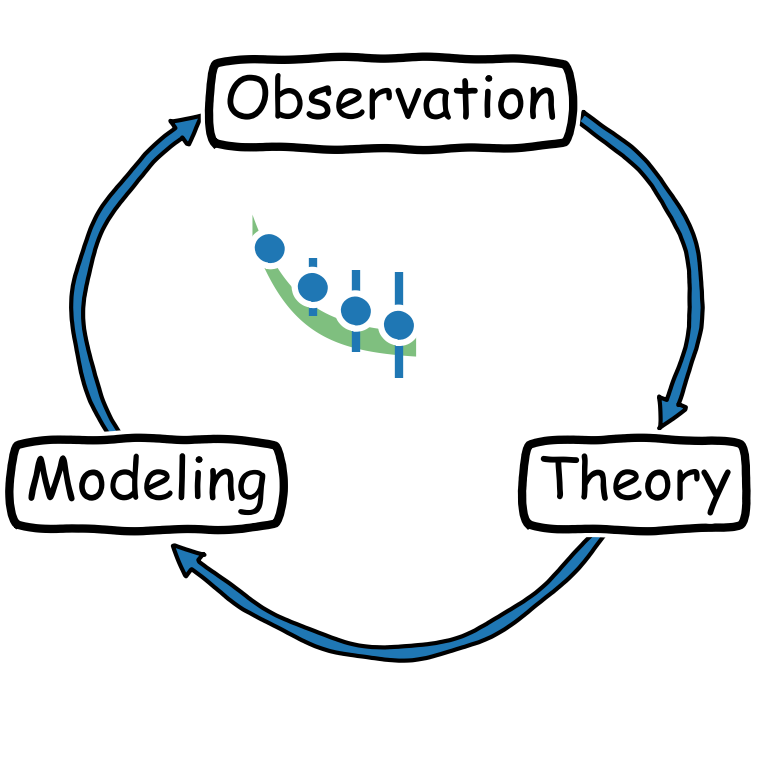
\includegraphics[width=0.4\linewidth]{fig/scientific_wheel_data.png}}

\vspace{6mm}



% !split
\paragraph{Statistical Inference.}

\begin{block_mdfboxadmon}[]
\begin{itemize}
\item Quantify the strength of inductive inferences from facts, in the form of data ($D$), and other premises, e.g.~models, to hypotheses about the phenomena producing the data.

\item Quantify via probabilities, or averages calculated using probabilities. Frequentists ($\mathcal{F}$) and Bayesians ($\mathcal{B}$) use probabilities very differently for this.

\item To the pioneers such as Bernoulli, Bayes and Laplace, a probability represented a \emph{degree-of-belief} or plausability: how much they thought that something as true based on the evidence at hand. This is the Bayesian approach.

\item To the 19th century scholars, this seemed too vague and subjective. They redefined probability as the \emph{long run relative frequency} with which an event occurred, given (infinitely) many repeated (experimental) trials.
\end{itemize}

\noindent
\end{block_mdfboxadmon} % title: 



% !split
\paragraph{Machine learning.}
The basic process illustrated in Fig.~\ref{fig-inference} is employed also in the field of machine learning. Here, the learning part might take place when confronting a large set of data with a machine learning algorithm, and the specific aim might be tasks such as classification or clusterization. 


\vspace{6mm}

% inline figure
\centerline{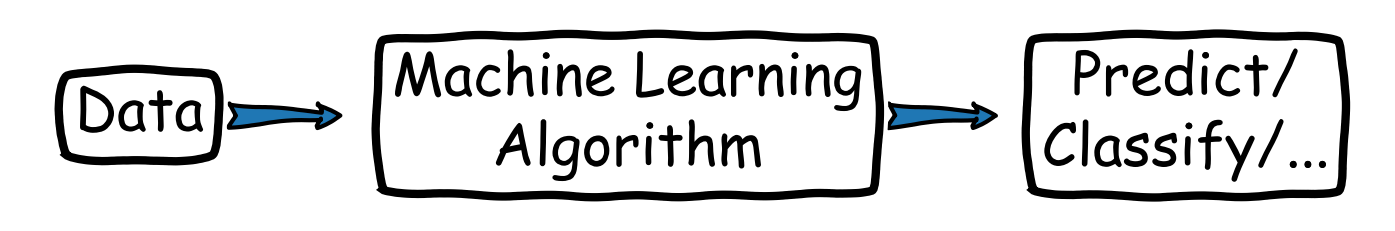
\includegraphics[width=0.8\linewidth]{fig/MLinference.png}}

\vspace{6mm}



Thus, we will be able to study statistical inference methods for learning from data and use them in scientific applications. In particular, we will use \textbf{Bayesian statistics}. Simultaneously we will slowly develop a deeper understanding and probabilistic interpretation of machine learning algorithms through a statistical foundation. 

% !split
\emph{Edwin Jaynes}, in his influential \href{{https://link.springer.com/chapter/10.1007%2F978-94-009-3049-0_1}}{How does the brain do plausible reasoning?}, wrote:

\begin{quote}
One of the most familiar facts of our experience is this: that there is such a thing as common sense, which enables us to do plausible reasoning in a fairly consistent way. People who have the same background of experience and the same amount of information about a proposition come to pretty much the same conclusions as to its plausibility. No jury has ever reached a verdict on the basis of pure deductive reasoning. Therefore the human brain must contain some fairly definite mechanism for plausible reasoning, undoubtedly much more complex than that required for deductive reasoning. But in order for this to be possible, there must exist consistent rules for carrying out plausible reasoning, in terms of operations so definite that they can be programmed on the computing machine which is the human brain.
\end{quote}


% !split
Jaynes went on to show that these ``consistent rules'' are just the rules of Bayesian probability theory, supplemented by Laplace's principle of indifference and, its generalization, Shannon's principle of maximum entropy. This key observation implies that a computer can be programmed to ``reason'', or, update probabilities based on data. Given some very minimal desiderata, the rules of Bayesian probability are the only ones which conform to what, intuitively, we recognize as rationality. Such probability update rules can be used recursively to impute causal relationships between observations, that is, a machine can be programmed to ``learn''.


\begin{summary_mdfboxadmon}[Summary]
Inference and machine learning, then, is the creative application of
Bayesian probability to problems of rational inference and causal
knowledge discovery based on data.
\end{summary_mdfboxadmon} % title: Summary



% !split
\section{Learning from data: A physicist's perspective}
\paragraph{How will this course be different from a computer science course?}
In this course we will focus in particular on the statistical foundation for being able to learn from data, in particular we will take the Bayesian viewpoint of extended logic. Although we aim for theoretical depth, we will still take a practical learning approach with many opportunities to apply the theories in practice using simple computer programs. 

% !split
However, being this ambitious in teaching a theoretical foundation means that there will be less time to cover the plethora of machine learning methods, or to find examples from a very wide list of subfields in physics. We believe that striving for theoretical depth and obtaining your own computational experience will give the best preparation for being able to apply the knowledge in new situations and for real problems that will be encountered in future studies and work. 

% !split
In particular, physics and astronomy students have a unique preparation:
\begin{itemize}
\item Strong background and experience with mathematical tools (linear algebra, multivariate calculus) needed for rigorous discussion of statistics.

\item Considerable training in general problem solution skills.
\end{itemize}

\noindent
Physics and astronomy research also has different needs:
\begin{itemize}
  \item Our data and models are often fundamentally different from those in typical computer science contexts.

  \item We ask different types of questions about our data, sometimes requiring new methods.

  \item We have different priorities for judging a ``good'' method: interpretability, error estimates, predictive power, etc.
\end{itemize}

\noindent
% !split
\paragraph{What is special about machine learning in physics and astronomy?}
\begin{itemize}
  \item We are data \textbf{producers}, not (only) data consumers:
\begin{itemize}

    \item Experimental design can (sometimes) be in our own control.

    \item Statistical errors on data can be quantified.

    \item Much efforts to understand systematic errors.
\end{itemize}

\noindent
\end{itemize}

\noindent
% !split
\begin{itemize}
  \item Our data represent measurements of physical processes:
\begin{itemize}

    \item Measurements often reduce to counting photons, etc, with known a-priori random errors.

    \item Dimensions and units are important.

    \item Experimental data comes with measurement errors that should be taken into account.

\end{itemize}

\noindent
  \item Our models are usually traceable to an underlying physical theory:
\begin{itemize}

    \item Models constrained by theory and previous observations.

    \item Parameter values often intrinsically interesting.

\end{itemize}

\noindent
  \item A parameter error estimate is just as important as its value:
\begin{itemize}

    \item Prefer methods that handle input data errors (weights) and provide output parameter error estimates.

\end{itemize}

\noindent
  \item In some experiments and scientific domains, the data sets are \emph{huge} (``Big Data'')
\end{itemize}

\noindent
% !split
% ======= Machine Learning =======
\section{Machine learning in science and society}

During the last two decades there has been a swift and amazing
development of Machine learning techniques and algorithms that impact
many areas in not only Science and Technology but also the Humanities,
Social Sciences, Medicine, Law, etc. Indeed, almost all possible
disciplines are affected. The applications are incredibly many, from self-driving
cars to solving high-dimensional differential equations or complicated
quantum mechanical many-body problems. Machine learning is perceived
by many as one of the main disruptive techniques nowadays. 

Statistics, Data science and Machine learning form important
fields of research in modern science.  They describe how to learn and
make predictions from data, as well as allowing us to extract
important correlations about physical process and the underlying laws
of motion in large data sets. The latter, big data sets, appear
frequently in essentially all disciplines, from the traditional
Science, Technology, Mathematics and Engineering fields to Life
Science, Law, education research, the Humanities and the Social
Sciences.

It has become more
and more common to see research projects on big data in for example
the Social Sciences where extracting patterns from complicated survey
data is one of many research directions.  Having a solid grasp of data
analysis and machine learning is thus becoming central to scientific
computing in many fields, and competences and skills within the fields
of machine learning and scientific computing are nowadays strongly
requested by many potential employers. The latter cannot be
overstated, familiarity with machine learning has almost become a
prerequisite for many of the most exciting employment opportunities,
whether they are in bioinformatics, life science, physics or finance,
in the private or the public sector. This author has had several
students or met students who have been hired recently based on their
skills and competences in scientific computing and data science, often
with marginal knowledge of machine learning.

Machine learning is a subfield of computer science, and is closely
related to computational statistics.  It evolved from the study of
pattern recognition in artificial intelligence (AI) research, and has
made contributions to AI tasks like computer vision, natural language
processing and speech recognition. Many of the methods we will study are also 
strongly rooted in basic mathematics and physics research. 

Ideally, machine learning represents the science of giving computers
the ability to learn without being explicitly programmed.  The idea is
that there exist generic algorithms which can be used to find patterns
in a broad class of data sets without having to write code
specifically for each problem. The algorithm will build its own logic
based on the data.  You should however always keep in mind that
machines and algorithms are to a large extent developed by humans. The
insights and knowledge we have about a specific system, play a central
role when we develop a specific machine learning algorithm. 

Machine learning is an extremely rich field, in spite of its young
age. The increases we have seen during the last three decades in
computational capabilities have been followed by developments of
methods and techniques for analyzing and handling large date sets,
relying heavily on statistics, computer science and mathematics.  The
field is rather new and developing rapidly. Popular software packages
written in Python for machine learning like
\href{{http://scikit-learn.org/stable/}}{Scikit-learn},
\href{{https://www.tensorflow.org/}}{Tensorflow},
\href{{http://pytorch.org/}}{PyTorch} and \href{{https://keras.io/}}{Keras}, all
freely available at their respective GitHub sites, encompass
communities of developers in the thousands or more. And the number of
code developers and contributors keeps increasing. Not all the
algorithms and methods can be given a rigorous mathematical
justification, opening up thereby large rooms for experimenting and
trial and error and thereby exciting new developments.  However, a
solid command of linear algebra, multivariate theory, probability
theory, statistical data analysis, understanding errors and Monte
Carlo methods are central elements in a proper understanding of many
of algorithms and methods we will discuss.



% !split
\subsection{Types of Machine Learning}


The approaches to machine learning are many, but are often split into
two main categories.  In \emph{supervised learning} we know the answer to a
problem, and let the computer deduce the logic behind it. On the other
hand, \emph{unsupervised learning} is a method for finding patterns and
relationship in data sets without any prior knowledge of the system.
Some authours also operate with a third category, namely
\emph{reinforcement learning}. This is a paradigm of learning inspired by
behavioral psychology, where learning is achieved by trial-and-error,
solely from rewards and punishment.

% !split
Another way to categorize machine learning tasks is to consider the
desired output of a system. What kind of inference are you hoping to see in your data? Is the aim to classify a result into categories, to predict a continuous value, or to simply observe patterns within the data? Let’s briefly introduce each class:

% !split
\begin{description}
\item[Classification algorithms:] 
  are used to predict whether a dataset’s outputs can be separated into separate classes, binary or otherwise. These output values are discrete and represent target classes. An example is to identify  digits based on pictures of hand-written ones. Classification algorithms undergo supervised training, which means they require labelled true output data in order to measure prediction accuracy.
\end{description}

\noindent
% !split
\begin{description}
\item[Clustering algorithms:] 
  can also be used for classification or simply to observe data patterns. By observing how the data is arranged within the feature space, clustering algorithms can utilize physical separation to create clusters. As such, some algorithms of this class don’t require output labels, making them unsupervised algorithms.
\end{description}

\noindent
% !split
\begin{description}
\item[Dimensionality reduction algorithms:] 
  focuses on decreasing the number of features from your dataset, preventing your models from “overfitting” or generalizing on previously unseen data. They are also unsupervised.
\end{description}

\noindent
% !split
\begin{description}
\item[Regression algorithms:] 
  Finding a functional relationship between an input data set and a reference data set. The goal is to construct a function that maps input data to continuous output values. These algorithms also require labelled true output data in order to measure prediction accuracy.
\end{description}

\noindent
% !split
In the natural sciences, where we often confront scientific models with observations, there is certainly a large interest in regression algorithms. However, there are also many examples where other classes of machine-learning algorithms are being used.

% !split
All methods have three main ingredients in common, irrespective of whether we deal with supervised or unsupervised learning. 

\begin{description}
\item[Data set:] 
  The first, and most important, one is normally our data set (which can be subdivided into training and test data). 

\item[Model:] 
  The second item is a model, which is normally a function of some parameters. The model reflects our knowledge of the system (or lack thereof). As an example, if we know that our data show a behavior similar to what would be predicted by a polynomial, fitting our data to a polynomial of some degree would then determine our model. 

\item[Cost function:] 
  The last ingredient is a so-called cost function, which allows us to present an estimate on how good our model is in reproducing the data it is supposed to describe.  
\end{description}

\noindent
% !split
\subsection{Choice of programming language}

Python plays a central role in the development of machine
learning techniques and tools for data analysis. In particular, given
the wealth of machine learning and data analysis libraries written in
Python, easy-to-use libraries with immediate visualization (and the
impressive galleries of existing examples), the popularity of the
Jupyter notebook framework (with the possibility to run \textbf{R} codes, or
simulation programs written in compiled languages), and much more made our choice of
programming language for this series of lectures easy. However,
since the focus here is not only on using existing Python libraries such
as \textbf{Scikit-Learn} or \textbf{Tensorflow}, but also on developing your own
algorithms and codes, we will as far as possible present many of these
algorithms as Python codes. 

The reason we also  mention compiled languages (like C, C++ or
Fortran), is that Python is still notoriously slow when we do not
utilize highly streamlined computational libraries 
written in compiled languages.  Therefore, analysis codes involving heavy Markov Chain Monte Carlo simulations and high-dimensional optimization of cost functions, tend to utilize C++/C or Fortran codes for the heavy lifting.

Presently thus, the community tends to let
code written in C++/C or Fortran do the heavy duty numerical
number crunching and leave the post-analysis of the data to the above
mentioned Python modules or software packages.  However, with the developments taking place in for example the Python community, and seen
the changes during the last decade, the above situation may change in the not too distant future. 

% !split
\subsection{Data handling, machine learning  and ethical aspects}

In most of the cases we will study, we will generate the data
to analyze ourselves. However, this does not hinder us from developing a sound
ethical attitude to the data we use, how we analyze the data and how
we handle it.

The most immediate and simplest possible ethical aspects deal with our
approach to the scientific process. Nowadays, with version control
software like \href{{https://git-scm.com/}}{Git} and various online
repositories like \href{{https://github.com/}}{Github},
\href{{https://about.gitlab.com/}}{Gitlab} etc, we can easily make our codes
and data sets we have used, freely and easily accessible to a wider
community. This helps us almost automagically in making our science
reproducible. The large open-source development communities involved
in say \href{{http://scikit-learn.org/stable/}}{Scikit-Learn},
\href{{https://www.tensorflow.org/}}{Tensorflow},
\href{{http://pytorch.org/}}{PyTorch} and \href{{https://keras.io/}}{Keras}, are
all excellent examples of this. The codes can be tested and improved
upon continuosly, helping thereby our scientific community at large in
developing data analysis and machine learning tools.  It is much
easier today to gain traction and acceptance for making your science
reproducible. From a societal stand, this is an important element
since many of the developers are employees of large public institutions like
universities and research labs.

However, this more mechanical aspect of the ethics of science (in
particular the reproducibility of scientific results) is something
which is obvious and everybody should do so as part of the dialectics of
science. 

Before we proceed, we should add a disclaimer. Even though
we may dream of computers developing some kind of higher learning
capabilities, at the end (even if the artificial intelligence
community keeps touting our ears full of fancy futuristic avenues), it is we, yes you reading these lines,
who end up constructing and instructing, via various algorithms, the
machine learning approaches. 

For self-driving vehicles, where the standard machine
learning algorithms discussed here enter into the software, there are
stages where we have to make choices. Yes, we, the humans who wrote
a program for a specific brand of a self-driving car.  As an example,
all carmakers have as their utmost priority the security of the
driver and the accompanying passengers. A famous European carmaker, which is
one of the leaders in the market of self-driving cars, had \textbf{if}
statements of the following type: suppose there are two obstacles in
front of you and you cannot avoid to collide with one of them. One of
the obstacles is a monstertruck while the other one is a kindergarten
class trying to cross the road. The self-driving car algo would then
opt for the hitting the small folks instead of the monstertruck, since
the likelihood of surving a collision with our future citizens, is
much higher.

This leads to serious ethical aspects. Why should we
opt for such an option? Who decides and who is entitled to make such
choices? Keep in mind that many of the algorithms you will encounter in
this series of lectures or hear about later, are indeed based on
simple programming instructions. And you are very likely to be one of
the people who may end up writing such a code. Thus, developing a
sound ethical attitude is much needed. The example of the self-driving cars is
just one of infinitely many cases where we have to make choices. When
you analyze data on economic inequalities, who guarantees that you are
not weighting some data in a particular way, perhaps because you dearly want a
specific conclusion which may support your political views?

We do not have the answers here, nor will we venture into a deeper
discussions of these aspects, but we want you think over these topics
in a more overarching way.  A statistical data analysis with its dry
numbers and graphs meant to guide the eye, does not necessarily
reflect the truth, whatever that is.  As a scientist, and after a
university education, you are supposedly a better citizen, with an
improved critical view and understanding of the scientific method, and
perhaps some deeper understanding of the ethics of science at
large. Use these insights. Be a critical citizen. You owe it to our
society.




% !split
% ======= A first data and machine learning encounter =======
\section{A first data and machine learning encounter}

A first demonstration of machine learning in physics is shown in the accompanying jupyter notebook. We will show some of the strengths of packages like \textbf{Scikit-Learn} in fitting nuclear binding energies to specific models using linear regression.

\subsection{Software and needed installations}

See the Getting started guide on the course web page.

% !split
% ======= Acknowledgements =======
\section{Acknowledgements}

The development of this course would not have been possible without the knowledge that has been gained through the study of several excellent textbooks, most of which are listed as recommended course literature. Here is a short list of those references that I have found the most influential and inspirational:

\begin{enumerate}
\item Phil Gregory, *``Bayesian Logical Data Analysis for the Physical Sciences''*, Cambridge University Press (2005).

\item E. T. Jaynes, *``Probability Theory: The Logic of Science''*, Cambridge University Press (2003).

\item David J.C. MacKay, *``Information Theory, Inference, and Learning Algorithms''*, Cambridge University Press (2005).

\item D.S. Sivia, *``Data Analysis : A Bayesian Tutorial''*, Oxford University Press (2006).
\end{enumerate}

\noindent
Even more importantly I would like to thank a number of colleagues and friends that have been paramount for the evolution of this course and for the
development of the course material that is an integral part. In particular, I am in deep gratitude to:

\begin{itemize}
\item Prof.~Richard Furnstahl, Ohio State University

\item Prof.~Morten Hjorth-Jensen, Oslo University and Michigan State University

\item Prof.~Daniel Phillips, Ohio University.
\end{itemize}

\noindent
The list of people that have contributed with ideas, discussions, or by generously sharing their knowledge is very long. Rather than taking the risk of forgetting someone, I would just like to say thank you all. I am truly thankful for being part of an academic environment in which ideas and efforts are shared rather than kept isolated.

The last statement extends obviously to the open source communities that make so many great computing tools publicly available. In this course we take much advantage of open-source python libraries.  

% ------------------- end of main content ---------------

% #ifdef PREAMBLE
\end{document}
% #endif

